%! TEX root = ../thesis.tex
\section{Wikipedia}
\label{pps:sec:wikipedia}

Wikipedia is a popular free online encyclopedia and arguably one of the most successful peer-production systems.
In this section, we apply our models to the French and Turkish editions of Wikipedia.

\subsection{Background \& Datasets}

The French Wikipedia is one of the largest Wikipedia editions.
At the time of writing, it ranks in third position both in terms of number of edits and number of users\footnote{%
	We chose the French edition over the English one because our computing infrastructure could not support the $\approx15$ TB needed to store the entire history of the English Wikipedia.
	The French edition contains roughly $5\times$ fewer edits.
}.
In order to obtain a complementary perspective, we also study the Turkish Wikipedia, which is roughly an order of magnitude smaller.
Interestingly, both the French and the Turkish editions score very highly on Wikipedia's \emph{depth} scale, a measure of collaborative quality~\citep{wikimedia2017depth}.

The Wikimedia Foundation releases periodically and publicly a database dump containing the successive revisions to all articles\footnote{%
	See: \url{https://dumps.wikimedia.org/}.}.
We use a dump that contains data starting from the beginning of the edition up to the fall of 2017:
The French Wikipedia contains edits between August 4, 2001, and September 2, 20017, and the Turkish Wikipedia between December 5, 2002, and October 1, 2017.

\subsubsection{Computation of Edit Quality}

On Wikipedia, any user's edit is immediately incorporated into the encyclopedia\footnote{Except for a small minority of protected articles.}.
Therefore, in order to obtain information about the quality of an edit, we have to consider the implicit signal given by subsequent edits to the same article.
If the changes introduced by the edit are preserved, it signals that the edit was beneficial, whereas if the changes are reverted, the edit likely had a negative effect.
A formalization of this idea is given by~\citet{adler2007content} and~\citet{druck2008learning};
see also~\citet{dealfaro2013content} for a concise explanation.
In this work, we essentially follow their approach.

Consider a particular article and denote by $v_k$ its $k$-th revision (\textit{i.e.}, the state of the article after the $k$-th edit).
Let $d(u, v)$ be the Levenshtein distance between two revisions~\citep{kruskal1983overview}.
We define the \emph{quality} of edit $k$ from the perspective of the article's state after $\ell \ge 1$ subsequent edits as
\begin{align*}
	q_{k \mid \ell} = \frac{1}{2} + \frac{d(v_{k-1}, v_{k + \ell}) - d(v_k, v_{k + \ell})}{2 d(v_{k-1}, v_k)}.
\end{align*}
By properties of distances, $q_{k \mid \ell} \in [0, 1]$.
Intuitively, the quantity $q_{k \mid \ell}$ captures the proportion of work done in edit $k$ that remains in revision $k + \ell$.
It can be understood as a \emph{soft} measure of whether edit $k$ has been reverted or not.
We compute the unconditional quality of the edit by averaging over multiple future revisions:
\begin{align}
	\label{pps:eq:wikiqual}
	q_k = \frac{1}{L} \sum_{\ell = 1}^L q_{k \mid \ell},
\end{align}
where $L$ is the minimum between the number of subsequent revisions of the article and $10$ (we empirically found that \num{10} revisions is enough to accurately assess the quality of an edit).
Note that even though $q_k$ is no longer binary, our models naturally extend to continuous-valued $q_k \in [0,1]$ (c.f. Section~\ref{pps:sec:learning}).

In practice, we observe that edit quality is bimodal and asymmetric.
Most edits have a quality close to either \num{0} or \num{1} and a majority of edits are of high quality.
The two rightmost columns of Table~\ref{pps:tab:wikidata} quantify this for the French and Turkish editions.

\subsubsection{Dataset Preprocessing}

We consider all edits to the pages in the main namespace (\textit{i.e.}, articles), including those from anonymous contributors identified by their IP address\footnote{%
	Note, however, that a large majority of edits are made by registered users (\num{82.7} \% and \num{76.6} \% for the French and Turkish editions, respectively).}.
Sequences of consecutive edits to an article by the same user are collapsed into a single edit in order to remove bias in the computation of edit quality~\citep{adler2007content}.
To evaluate methods in a realistic setting, we split the data into a training set containing the first \num{90} \% of edits, and we report results on an independent validation set containing the remaining \num{10} \%.
%\footnote{%
%The cutoff dates are May 2\textsuperscript{nd}, 2016 (French edition) and July 29\textsuperscript{th}, 2016 (Turkish edition).}.
Note that the quality is computed based on subsequent revisions of an article:
In order to guarantee that the two sets are truly independent, we make sure that we never use any revisions from the validation set to compute the quality of edits in the training set.
%Finally, we remove edits whose quality cannot be assessed reliably, \textit{i.e.}, those that have $L < 2$ in \eqref{pps:eq:wikiqual}.
A short summary of the data statistics after preprocessing is provided in Table~\ref{pps:tab:wikidata}.

\begin{table}
	\centering
	\caption{Summary statistics of Wikipedia datasets after preprocessing.}
	\label{pps:tab:wikidata}
	\begin{tabular}{lrrrrr}
		\toprule
		Edition              & \# users $N$  & \# articles $M$ & \# edits       & $q < 0.2$    & $q > 0.8$    \\
		\midrule
		French  (2001--2017) & \num{5460745} & \num{1932810}   & \num{65430838} & \num{6.4}\%  & \num{72.2}\% \\
		Turkish (2002--2017) & \num{1360076} & \num{310991}    & \num{8768258}  & \num{11.6}\% & \num{60.5}\% \\
		\bottomrule
	\end{tabular}
\end{table}


\subsection{Evaluation}

In order to facilitate the comparison of our method with competing approaches, we evaluate the performance on a binary classification task consisting of predicting whether an edit is of poor quality.
To this end, we assign binary labels to all edits in the validation set: the label \emph{bad} is assigned to every edit with $q < 0.5$, and the label \emph{good} is assigned to all edits with $q \ge 0.5$.
The predictions of the classifier might help Wikipedia administrators to identify edits of low quality;
these edits might then be sent to domain experts for review.

As discussed in Section~\ref{pps:sec:models}, we consider two versions of our model.
The first one, \textsc{interank} \emph{basic}, simply learns scalar user skills and article difficulties.
The second one, \textsc{interank} \emph{full}, additionally includes a latent embedding of dimension $D = 20$ for each user and article.

\subsubsection{Competing Approaches}
\label{pps:sec:wikicompeting}
To set our results in context, we compare them to those obtained with four different baselines.

\paragraph{Average}
The first approach always outputs the marginal probability of a bad edit in the training set, \textit{i.e.},
\begin{align*}
	p = \frac{\text{\# bad edits in training set}}{\text{\# edits in training set}}
\end{align*}
This is a trivial baseline, and it gives an idea of what results we should expect to achieve without any additional information on the user, article or edit.

\paragraph{User-Only}
The second approach models the outcome of an edit using only the user's identity.
In short, the predictor learns skills $\{s_u \mid u = 1, \ldots, N\}$ and a global offset $b$ such that, for each user $u$, the probability
\begin{align*}
	\Prob{u} = \frac{1}{1 + \exp[- (s_u + b)]}
\end{align*}
maximizes the likelihood of that user's edits in the training set.
This baseline predictor is representative of user reputation systems such as that of~\citet{adler2007content}.

\paragraph{GLAD}
In the context of crowdsourcing,~\citet{whitehill2009whose} propose the GLAD model that postulates that
\begin{align*}
	\Prob{u \succ i} = \frac{1}{1 + \exp(- s_u / d_i)},
\end{align*}
where $s_u \in \mathbf{R}$ and $d_i \in \mathbf{R}_{>0}$.
This reflects a different assumption on the interplay between user skill and item difficulty: under their model, an item with a large difficulty value makes every user's skill more ``diffuse''.
In order to make the comparison fair, we add a global offset parameter $b$ to the model (similarly to \textsc{interank} and the user-only baseline).

\paragraph{ORES reverted}
The fourth approach is a state-of-the-art classifier developed by researchers at the Wikimedia Foundation as part of Wikipedia's Objective Revision Evaluation Service~\citep{wikimedia2015artificial}.
We use the two classification models specifically developed for the French and Turkish editions.
Both models use over \num{80} content-based and system-based features extracted from the user, the article and the edit to predict whether the edit will be reverted, a target which essentially matches our operational definition of \emph{bad} edit.
Features include the number of vulgar words introduced by the edit, the length of the article and of the edit, etc.
This predictor is representative of specialized, domain-specific approaches to modeling edit quality.

\subsubsection{Results}

Table~\ref{pps:tab:wikiperf} presents the average log-likelihood and the area under the precision-recall curve (AUPRC) for each method.
\textsc{interank} \emph{full} has the highest average log-likelihood of all models, meaning that its predictive probabilities are well calibrated with respect to the validation data.

\begin{table}
	\centering
	\caption{Predictive performance on the \emph{bad edit} classification task for the French and Turkish editions of Wikipedia.
		The best performance is highlighted in bold.}
	\label{pps:tab:wikiperf}
	\begin{tabular}{llrr}
		\toprule
		Edition & Model                          & Avg. log-likelihood   & AUPRC                \\
		\midrule
		French  & \textsc{interank} \emph{basic} & \num{-0.339}          & \num{0.399}          \\
		        & \textsc{interank} \emph{full}  & \textbf{\num{-0.336}} & \num{0.413}          \\
		\addlinespace
		        & Average                        & \num{-0.389}          & \num{0.131}          \\
		        & User-only                      & \num{-0.346}          & \num{0.313}          \\
		        & GLAD                           & \num{-0.344}          & \num{0.369}          \\
		        & ORES reverted                  & \num{-0.469}          & \textbf{\num{0.453}} \\
		\midrule
		Turkish & \textsc{interank} \emph{basic} & \num{-0.380}          & \num{0.494}          \\
		        & \textsc{interank} \emph{full}  & \textbf{\num{-0.379}} & \num{0.503}          \\
		\addlinespace
		        & Average                        & \num{-0.461}          & \num{0.168}          \\
		        & User-only                      & \num{-0.390}          & \num{0.410}          \\
		        & GLAD                           & \num{-0.387}          & \num{0.471}          \\
		        & ORES reverted                  & \num{-0.392}          & \textbf{\num{0.552}} \\
		\bottomrule
	\end{tabular}
\end{table}

Figure~\ref{pps:fig:wikipr} presents the precision-recall curves for all methods.
The analysis is qualitatively similar for both Wikipedia editions.
All non-trivial predictors perform similarly in the high-recall regime, but present significant differences in the high-precision regime, on which we will focus.
The ORES predictor performs the best.
\textsc{interank} comes second, reasonably close behind ORES, and the \emph{full} variant has a small edge over the \emph{basic} variant.
GLAD is next, and the user-only baseline is far behind.
This shows that
\begin{enuminline}
	\item incorporating information about the article being edited is crucial for achieving a good performance on a large portion of the precision-recall trade-off, and
	\item modeling the outcome probability by using the \emph{difference} between skill and difficulty (\textsc{interank}) is better than by using the \emph{ratio} (GLAD).
\end{enuminline}

\begin{figure}
	\centering
	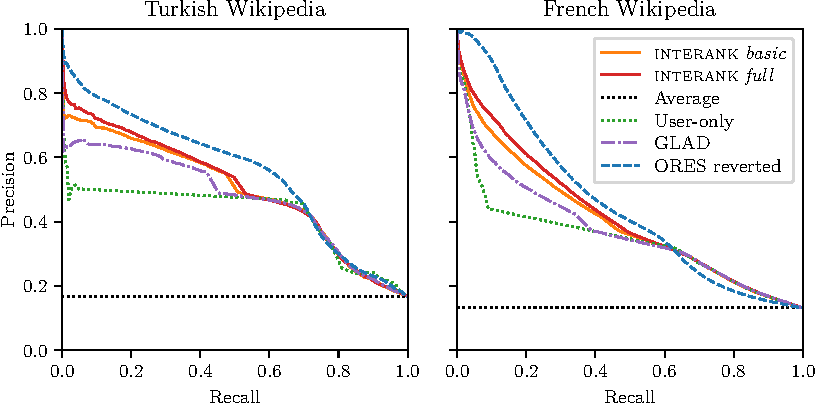
\includegraphics{pps-wikipedia-pr}
	\caption{Precision-recall curves on the \emph{bad edit} classification task for the Turkish and French editions of Wikipedia.}
	\label{pps:fig:wikipr}
\end{figure}

We also note that in the validation set, approximately \num{20} \% (\num{15} \%) of edits are made by users (respectively, on articles) that are never encountered in the training set (the numbers are similar in both editions).
% Explicit "default predictions"?
In these cases, \textsc{interank} reverts to average predictions, whereas content-based methods can take advantage of other features of the edit to make an informed prediction.
In order to explore this \emph{cold-start} effect in more detail, we group users and articles into bins based on the number of times they appear in the training set, and we compute the average log-likelihood of validation examples separately for each bin.
Figure~\ref{pps:fig:wikics} presents the results for the French edition;
the results for the Turkish edition are similar.
Clearly, predictions for users and articles present in the training set are significantly better.
In a practical deployment, several methods can help to address this issue~\citep{schein2002methods, lam2008addressing, levi2012finding}.
A thorough investigation of ways to mitigate the cold-start problem is beyond the scope of this work.

\begin{figure}
	\centering
	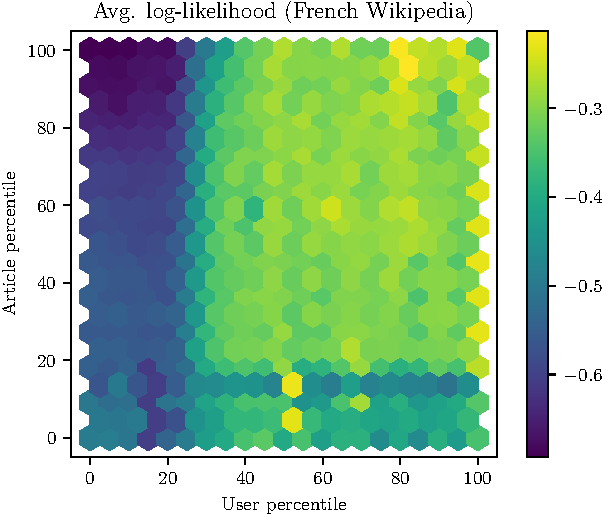
\includegraphics{pps-wikipedia-cs}
	\caption{Average log-likelihood as a function of the number of observations of the user and item in the training set of the French Wikipedia.}
	\label{pps:fig:wikics}
\end{figure}

In summary, we observe that our model, which incorporates the articles' identity, is able to bridge the gap between user-only prediction approach and a specialized predictor (ORES reverted).
Furthermore, modeling the interaction between user and article (\textsc{interank} \emph{full}) is beneficial and helps further improve predictions, particularly in the high-precision regime.

\subsection{Interpretation of Model Parameters}

The parameters of \textsc{interank} models, in addition to being predictive of edit outcomes, are also very interpretable.
In the following, we demonstrate how they can surface interesting characteristics of the peer-production system.

\subsubsection{Controversial Articles}
Intuitively, we expect an article $i$ whose difficulty parameter $d_i$ is large to deal with topics that are potentially controversial.
We focus on the French Wikipedia and explore a list of the ten most controversial articles given by~\citet{yasseri2014most}.
In this 2014 study, the authors identify controversial articles by using an ad-hoc methodology.
Table~\ref{pps:tab:wikicontrov} presents, for each article identified by~\citeauthor{yasseri2014most}, the percentile of the corresponding difficulty parameter $d_i$ learned by \textsc{interank} \emph{full}.
We analyze these articles approximately four years later, but the model still identifies them as some of the most difficult ones.
Interestingly, the article on Sigmund Freud, which has the lowest difficulty parameter of the list, has become a \emph{featured} article since~\citeauthor{yasseri2014most}'s analysis---a distinction awarded only to the most well-written and neutral articles.

\begin{table}
	\centering
	\caption{The ten most controversial articles on the French Wikipedia according to~\citet{yasseri2014most}.
		For each article $i$, we indicate the percentile of its corresponding parameter $d_i$.}
	\label{pps:tab:wikicontrov}
	\begin{tabular}{rlr}
		\toprule
		Rank & Title                       & Percentile of $d_i$ \\
		\midrule
		1    & Ségolène Royal              & \num{99.840} \%     \\
		2    & Unidentified flying object  & \num{99.229} \%     \\
		3    & Jehovah's Witnesses         & \num{99.709} \%     \\
		4    & Jesus                       & \num{99.953} \%     \\
		5    & Sigmund Freud               & \num{97.841} \%     \\
		6    & September 11 attacks        & \num{99.681} \%     \\
		7    & Muhammad al-Durrah incident & \num{99.806} \%     \\
		8    & Islamophobia                & \num{99.787} \%     \\
		9    & God in Christianity         & \num{99.712} \%     \\
		10   & Nuclear power debate        & \num{99.304} \%     \\
		\addlinespace
		     & \emph{Median}               & \num{99.710} \%     \\
		\bottomrule
	\end{tabular}
\end{table}

\subsubsection{Latent Factors}

Next, we turn our attention to the parameters $\{ \bm{y}_i \}$.
These parameters can be thought of as an embedding of the articles in a latent space of dimension $D = 20$.
As we learn a model that maximizes the likelihood of edit outcomes, we expect these embeddings to capture latent article features that explain edit outcomes.
In order to extract the one or two directions that explain most of the variability in this latent space, we apply principal component analysis~\citep{bishop2006pattern} to the matrix $\bm{Y} = [\bm{y}_i]$.

In Table~\ref{pps:tab:wikitrlatent}, we consider the Turkish Wikipedia and list a subset of the \num{20} articles with the highest and lowest coordinates along the first principal axis of $\bm{Y}$.
We observe that this axis seems to distinguish articles about popular culture from those about ``high culture'' or timeless topics.
This discovery supports the hypothesis that users have a propensity to successfully edit \emph{either} popular culture \emph{or} high-culture articles on Wikipedia, but not \emph{both}.

\begin{table}
	\centering
	\caption{A selection of articles of the Turkish Wikipedia among the top-\num{20} highest and lowest coordinates along the first principal axis of the matrix $\bm{Y}$.}
	\label{pps:tab:wikitrlatent}
	\begin{tabular}{lp{4.8in}}
		\toprule
		Direction & Titles                       \\
		\midrule
		Lowest    &
		Harry Potter's magic list,
		List of programs broadcasted by Star TV,
		Bursaspor 2011-12 season,
		Kral Pop TV Top 20,
		Death Eater,
		Heroes (TV series),
		List of programs broadcasted by TV8,
		Karadayı,
		Show TV,
		List of episodes of Kurtlar Vadisi Pusu. \\
		Highest   &
		Seven Wonders of the World,
		Thomas Edison,
		Cell,
		Mustafa Kemal Atatürk,
		Albert Einstein,
		Democracy,
		Isaac Newton,
		Mehmed the Conqueror,
		Leonardo da Vinci,
		Louis Pasteur.                           \\
		\bottomrule
	\end{tabular}
\end{table}

Finally, we consider the French Wikipedia.
Once again, we apply principal component analysis to the matrix $\bm{Y}$ and keep the first two dimensions.
We select the \num{20} articles with the highest and lowest coordinates along the first two principal axes\footnote{%
	Interestingly, the first dimension has a very similar interpretation to that obtained on the Turkish edition: it can also be understood as separating popular culture from high culture.}.
A two-dimensional $t$-SNE plot~\citep{vandermaaten2008visualizing} of the 80 articles selected using PCA is displayed in Figure~\ref{pps:fig:wikifrlatent}.
% "teen culture" is too colloquial? Maybe "teenager culture" or "youth culture"?
The plot enables identifying meaningful clusters of related articles, such as articles about tennis players, French municipalities, historical figures, and TV or teen culture.
These articles are representative of the latent dimensions that separate editors the most:
a user skilled in editing pages about ancient Greek mathematicians might be less skilled in editing pages about \emph{anime}, and vice versa.

\begin{figure}
	\centering
	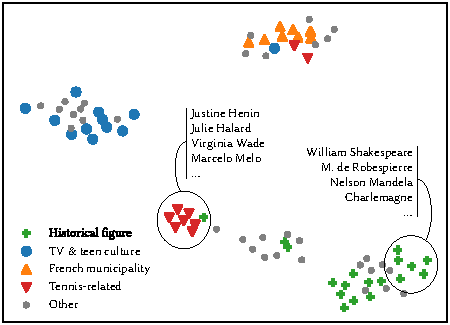
\includegraphics[width=\linewidth*3/4]{pps-wikipedia-latentfact}
	\caption{$t$-SNE visualization of 80 articles of the French Wikipedia with highest and lowest coordinates along the first and second principal axes of the matrix $\bm{Y}$.}
	\label{pps:fig:wikifrlatent}
\end{figure}
